% =====================================================================
%  Chapitre 1 -- partie c : formalisation, optimisation, evaluation
%  Public : Licence 3 SDIA (maths, Python, statistique acquis)
% =====================================================================

\begin{frame}{Formaliser : espace d'hypothèses et perte}
\begin{columns}[t]
\begin{column}{0.50\textwidth}
On dispose de $n$ exemples $\{(x_i, y_i)\}_{i=1}^n$, avec
$x_i \in \R^d$ et $y_i \in \mathcal{Y}$.

\vspace{1mm}
Un \textbf{modèle} est une fonction $f_\theta$ choisie dans une famille
$\mathcal{H}$ :
\[
  \mathcal{H} = \{\, f_\theta : \theta \in \Theta \,\}.
\]
\textbf{Apprendre} $=$ trouver $\theta$ qui minimise une \textbf{perte}
moyenne :
\[
  \hat\theta = \argmin_{\theta \in \Theta}\;
  \frac{1}{n}\sum_{i=1}^{n} L\big(y_i, f_\theta(x_i)\big).
\]
\end{column}
\begin{column}{0.46\textwidth}
\begin{kbox}[Deux mots à ne pas confondre]
\textbf{Famille} $\mathcal{H}$ : l'ensemble des modèles possibles
(linéaires, arbres, réseaux\ldots).\\[2pt]
\textbf{Paramètres} $\theta$ : ce qui est ajusté à l'intérieur de la famille.
\end{kbox}
\begin{wbox}[Conséquence]
Choisir une famille trop pauvre rend le problème insoluble, quelle que soit la
qualité de l'optimisation.
\end{wbox}
\end{column}
\end{columns}
\end{frame}

\begin{frame}{Risque réel et risque empirique}
\begin{center}
\[
  R(\theta) \;=\; \E_{(x,y)\sim P}\big[L(y, f_\theta(x))\big]
  \qquad\text{vs}\qquad
  \hat R_n(\theta) \;=\; \frac{1}{n}\sum_{i=1}^{n} L(y_i, f_\theta(x_i))
\]
\end{center}
\begin{columns}[t]
\begin{column}{0.48\textwidth}
\begin{itemize}
  \item $R(\theta)$ : performance sur la \textbf{population} --- inaccessible.
  \item $\hat R_n(\theta)$ : performance sur l'échantillon --- calculable.
  \item On minimise $\hat R_n$ en espérant que $R$ suive.
\end{itemize}
\end{column}
\begin{column}{0.48\textwidth}
\begin{wbox}[Tout le cours tient dans cet écart]
Plus $\mathcal{H}$ est riche, plus $\hat R_n$ peut être rendu petit --- et plus
l'écart avec $R$ risque d'être grand. C'est le surapprentissage, énoncé
mathématiquement.
\end{wbox}
\end{column}
\end{columns}
\end{frame}

\begin{frame}{Comment on minimise : descente de gradient}
\begin{columns}[t]
\begin{column}{0.50\textwidth}
\centering
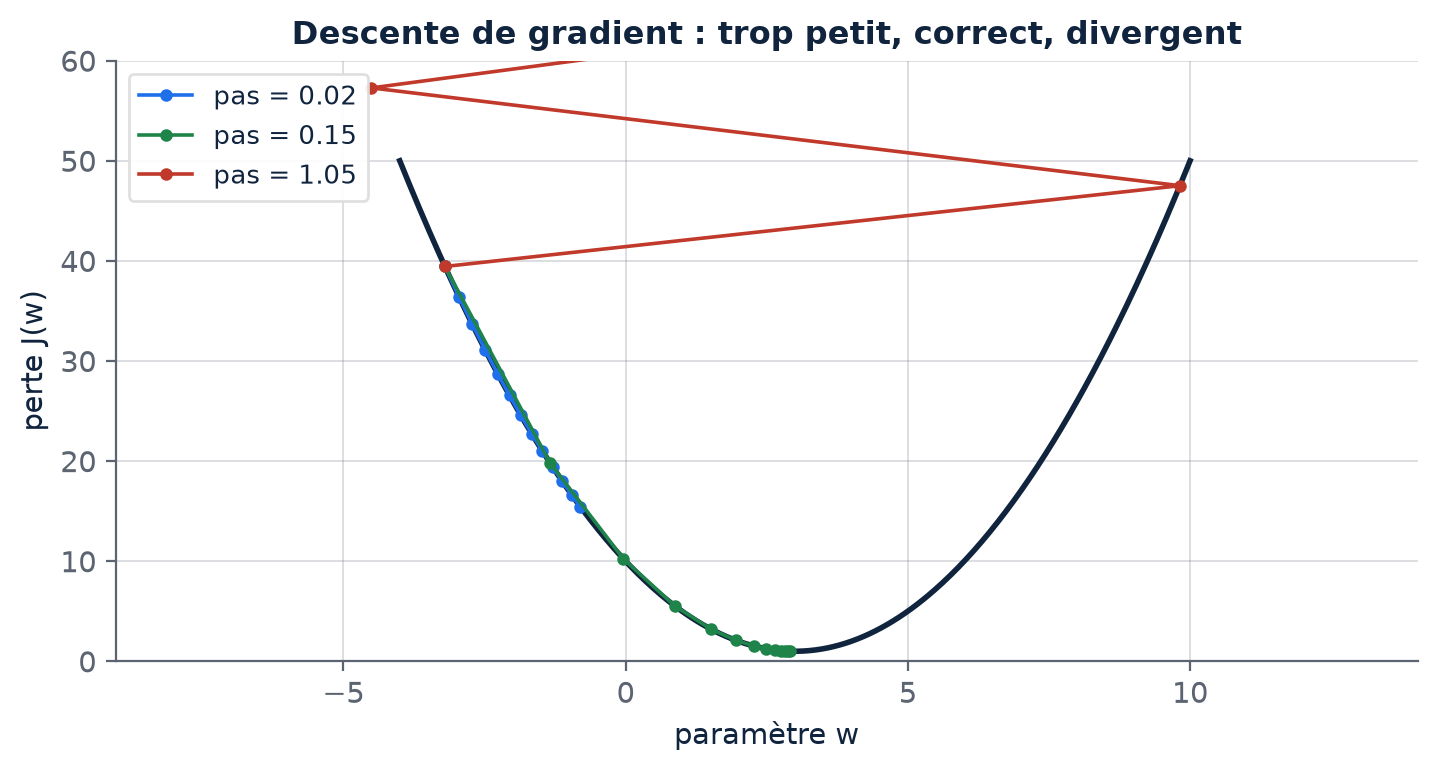
\includegraphics[height=0.30\textheight,keepaspectratio]{g12_descente_gradient.png}
\end{column}
\begin{column}{0.46\textwidth}
\[
  \theta_{t+1} = \theta_t - \eta\,\nabla_\theta \hat R_n(\theta_t)
\]
\begin{itemize}
  \item $\eta$ : pas d'apprentissage.
  \item Trop petit : convergence interminable. Trop grand : divergence.
\end{itemize}
\begin{solbox}[Mesuré sur $J(w)=(w-3)^2+1$]
$\eta=0{,}02$ : approche monotone. $\eta=0{,}15$ : converge en 4 pas.
$\eta=1{,}05$ : $-3{,}2 \to 9{,}8 \to -4{,}5 \to 11{,}3$ : divergence.
\end{solbox}
\end{column}
\end{columns}
\end{frame}

\begin{frame}{Les pertes usuelles, et ce qu'elles impliquent}
\begin{center}
\footnotesize
\begin{tabular}{@{}p{0.16\textwidth}p{0.30\textwidth}p{0.42\textwidth}@{}}
\toprule
\textbf{Perte} & \textbf{Formule} & \textbf{Quand l'utiliser} \\
\midrule
Quadratique & $\frac{1}{n}\sum (y_i-\hat y_i)^2$ & régression, bruit gaussien ;
les grandes erreurs pèsent double \\
Absolue & $\frac{1}{n}\sum |y_i-\hat y_i|$ & régression robuste aux
valeurs aberrantes \\
Entropie croisée & $-\frac{1}{n}\sum \log p_\theta(y_i \given x_i)$ &
classification probabiliste \\
Hinge & $\frac{1}{n}\sum \max(0, 1-y_i f(x_i))$ & marge (SVM) \\
\bottomrule
\end{tabular}
\end{center}
\vspace{1.5mm}
\begin{kbox}[Le choix de la perte est un choix de modélisation]
La perte quadratique suppose un bruit symétrique de variance constante ; sur
des données à outliers, elle tire le modèle vers les extrêmes.
\end{kbox}
\end{frame}

\begin{frame}{Activité : risque empirique à la main (8 min)}
\begin{columns}[t]
\begin{column}{0.46\textwidth}
\small
\begin{tabular}{@{}rrr@{}}
\toprule
$i$ & $y_i$ & $\hat y_i$ \\
\midrule
1 & 100 & 90 \\
2 & 150 & 120 \\
3 & 80  & 100 \\
4 & 200 & 180 \\
\bottomrule
\end{tabular}
\vspace{2mm}

Calculez $\hat R_4$ pour la perte quadratique, puis pour la perte absolue.
\end{column}
\begin{column}{0.50\textwidth}
\begin{solbox}[Corrigé]
Erreurs : $-10$, $-30$, $+20$, $-20$.

\vspace{1mm}
Quadratique : $(100+900+400+400)/4 = \mathbf{450}$ ;\\[1pt]
RMSE $=\sqrt{450}\approx\mathbf{21{,}2}$.

\vspace{1mm}
Absolue : $(10+30+20+20)/4 = \mathbf{20}$.
\end{solbox}
\begin{kbox}[Lecture]
Les deux pertes ne classent pas les mêmes modèles : l'erreur de 30 pèse
9 fois plus que celle de 10 en quadratique, 3 fois plus en absolue.
\end{kbox}
\end{column}
\end{columns}
\end{frame}

\begin{frame}{Plus de données : la courbe d'apprentissage}
\begin{columns}[t]
\begin{column}{0.52\textwidth}
\centering
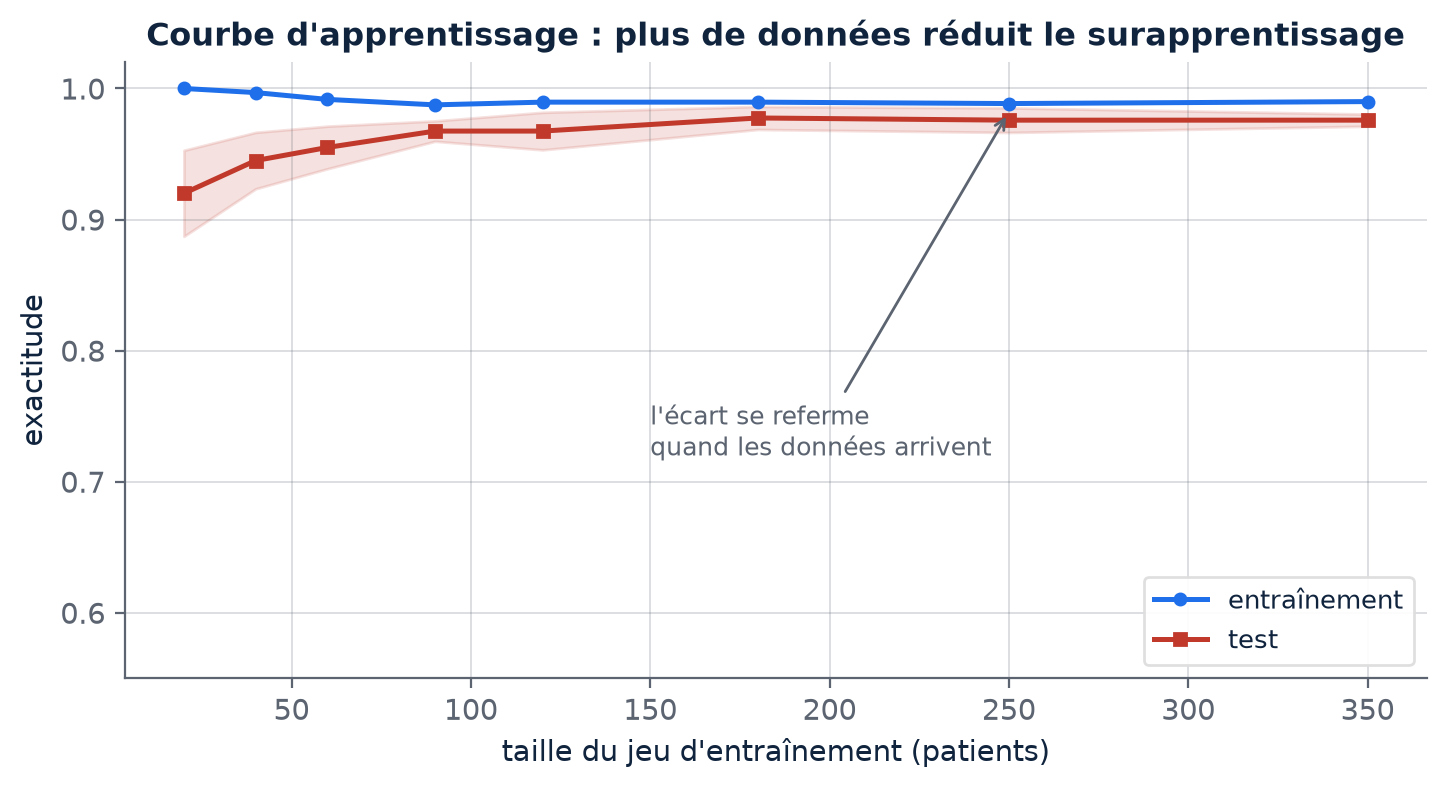
\includegraphics[height=0.34\textheight,keepaspectratio]{g09_courbe_apprentissage.png}
\end{column}
\begin{column}{0.44\textwidth}
\begin{itemize}
  \item À 20 patients : entraînement $100\,\%$, test faible.
  \item À 350 patients : l'écart tombe à \textbf{0,014}.
  \item L'erreur de test plafonne : c'est le bruit irréductible.
\end{itemize}
\begin{kbox}[À retenir]
Si l'écart se referme avec $n$, il manquait des données. S'il ne se referme
pas, c'est la famille de modèles qu'il faut changer.
\end{kbox}
\end{column}
\end{columns}
\end{frame}

\begin{frame}{Cinq schémas de validation croisée}
\begin{center}
\footnotesize
\begin{tabular}{@{}p{0.20\textwidth}p{0.36\textwidth}p{0.34\textwidth}@{}}
\toprule
\textbf{Schéma} & \textbf{Principe} & \textbf{Quand l'utiliser} \\
\midrule
$K$-fold & $K$ plis, chacun sert une fois de validation & cas général, données
i.i.d. \\
Stratifié & proportions de classes conservées dans chaque pli & classification
déséquilibrée \\
Groupé & toutes les observations d'un individu dans le même pli & visites
répétées, même patient, même site \\
Temporel & entraînement sur le passé, validation sur la suite & séries,
prévision, fraude \\
Leave-one-out & $K=n$, un point de côté à chaque fois & très petits jeux,
coût prohibitif sinon \\
\bottomrule
\end{tabular}
\end{center}
\vspace{1.5mm}
\begin{wbox}[Le choix n'est pas cosmétique]
Même modèle, mêmes données : $58\,\%$ ou $90\,\%$ selon le découpage.
\end{wbox}
\end{frame}

\begin{frame}{Validation groupée : quand un individu revient}
\vspace{5mm}
\begin{columns}[t]
\begin{column}{0.44\textwidth}
\centering\vspace{0pt}
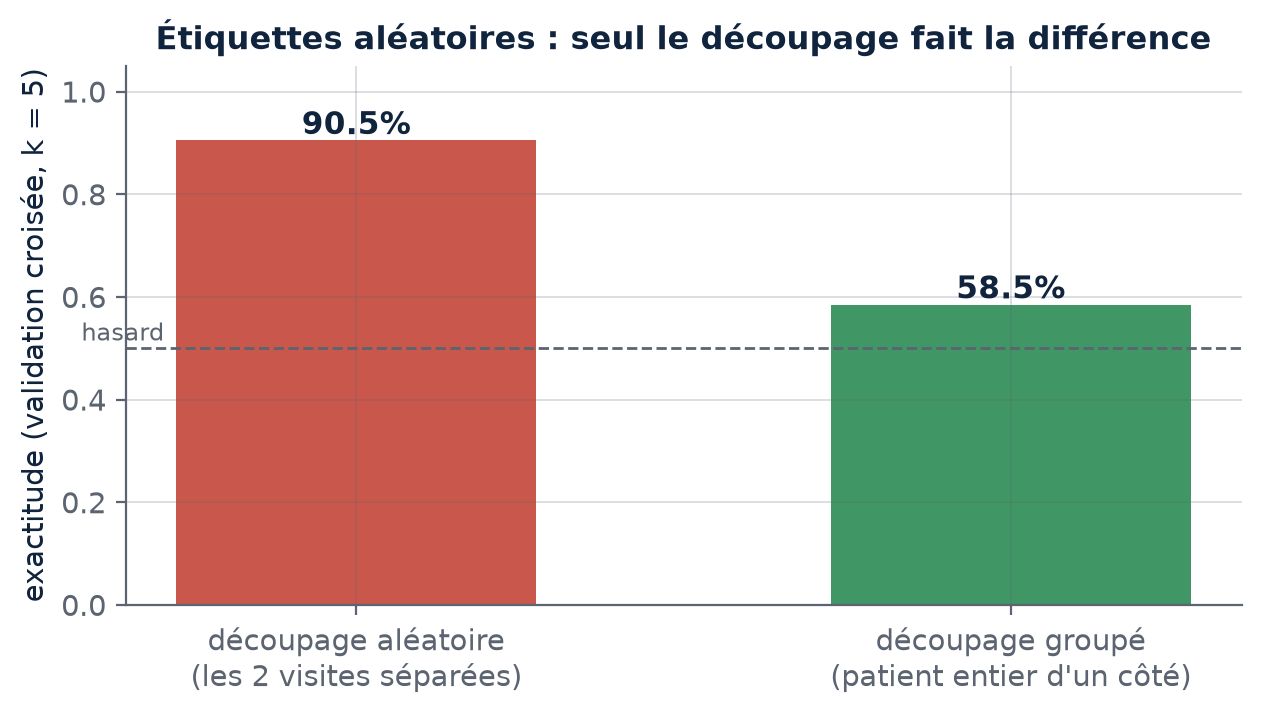
\includegraphics[height=0.27\textheight,keepaspectratio]{g13_validation_groupee.png}
\end{column}
\begin{column}{0.54\textwidth}
\begin{itemize}
  \item 200 patients, 2 visites chacun, \textbf{étiquettes aléatoires par
        patient}.
  \item Découpage aléatoire : \textbf{90,5 \%}.
  \item Découpage groupé : \textbf{58,5 \%}.
  \item Écart : \textbf{+32 points}, sans aucune information apprise.
\end{itemize}
\begin{wbox}[Le mécanisme]
Le modèle reconnaît la \textbf{signature} du patient déjà vu : il n'apprend
pas la maladie, il reconnaît la personne.
\end{wbox}
\end{column}
\end{columns}
\end{frame}

\begin{frame}{Deux découpages que le hasard ne remplace pas}
\begin{columns}[t]
\begin{column}{0.48\textwidth}
\begin{ebox}[Temporel]
Séries, prévision, fraude : on entraîne sur le passé et on teste sur le futur.
\[
  \underbrace{t_1,\dots,t_k}_{\text{train}}\;
  \underbrace{t_{k+1},\dots,t_n}_{\text{test}}
\]
Mélanger les dates fait fuiter l'avenir.
\end{ebox}
\end{column}
\begin{column}{0.48\textwidth}
\begin{ebox}[Stratifié]
Classification déséquilibrée : on conserve la proportion des classes dans
chaque pli.
\[
  \frac{n_{\text{positifs}}}{n}\;\text{identique dans chaque partition}
\]
Sans cela, un pli peut ne contenir aucun cas rare.
\end{ebox}
\end{column}
\end{columns}
\vspace{1.5mm}
\begin{wbox}[Règle]
Le découpage doit reproduire les conditions d'utilisation réelles. Un split
aléatoire sur des données ordonnées ou groupées est une fuite, même sans
variable explicite.
\end{wbox}
\end{frame}

\begin{frame}{Combien de plis ? Répéter ou laisser un seul point de côté}
\begin{columns}[t]
\begin{column}{0.46\textwidth}
\centering
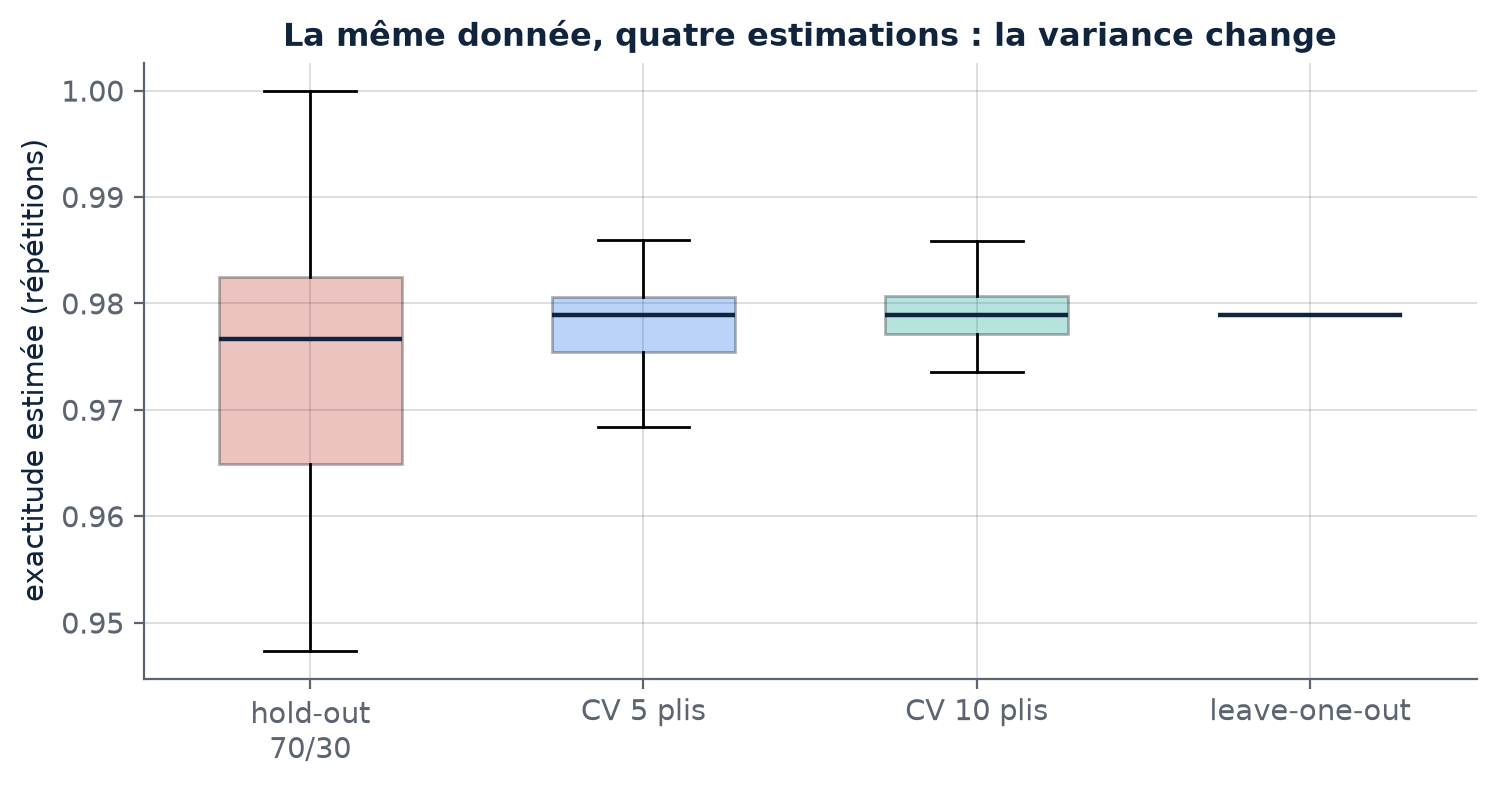
\includegraphics[height=0.34\textheight,keepaspectratio]{g10_variabilite.png}
\end{column}
\begin{column}{0.52\textwidth}
\small
\begin{tabular}{@{}lr@{}}
\toprule
\textbf{Schéma} & \textbf{Écart-type} \\
\midrule
hold-out 70/30 & $0{,}0105$ \\
$K=5$ & $0{,}0034$ \\
$K=10$ & $0{,}0024$ \\
leave-one-out & déterministe \\
\bottomrule
\end{tabular}
\vspace{2mm}
\begin{itemize}
  \item $K=5$ : compromis coût / stabilité.
  \item $K=10$ : plus stable, cinq fois plus coûteux.
  \item $K=n$ : sans biais de découpage, mais sensible aux points influents.
  \item \textbf{Répéter} un $K$-fold avec d'autres tirages mesure la variabilité
        du découpage lui-même.
\end{itemize}
\end{column}
\end{columns}
\end{frame}

\begin{frame}{Évaluer une classification : au-delà de l'exactitude}
\begin{columns}[t]
\begin{column}{0.42\textwidth}
\small
\begin{tabular}{@{}lrr@{}}
\toprule
 & \textbf{prédit 0} & \textbf{prédit 1} \\
\midrule
\textbf{réel 0} & 1\,720 & 180 \\
\textbf{réel 1} & 20    & 80 \\
\bottomrule
\end{tabular}
\vspace{2mm}

{\footnotesize $n=2\,000$, prévalence 5 \%.}
\end{column}
\begin{column}{0.54\textwidth}
\begin{solbox}[Trois calculs]
Exactitude $=\dfrac{1720+80}{2000}=\mathbf{90\ \%}$\\[2pt]
Précision $=\dfrac{80}{80+180}=\mathbf{30{,}8\ \%}$\\[2pt]
Rappel $=\dfrac{80}{80+20}=\mathbf{80\ \%}$\\[2pt]
$F_1=\dfrac{2\cdot 80}{2\cdot 80+180+20}=\mathbf{44{,}4\ \%}$
\end{solbox}
\end{column}
\end{columns}
\vspace{1mm}
\begin{kbox}[Choisir la métrique, c'est choisir ce que coûte une erreur]
Rater un malade coûte plus qu'une fausse alerte : on privilégie le rappel.
Inonder le service d'alertes inutiles : on privilégie la précision.
\end{kbox}
\end{frame}

\begin{frame}{Quand l'exactitude ment : le déséquilibre}
\begin{columns}[t]
\begin{column}{0.44\textwidth}
\centering
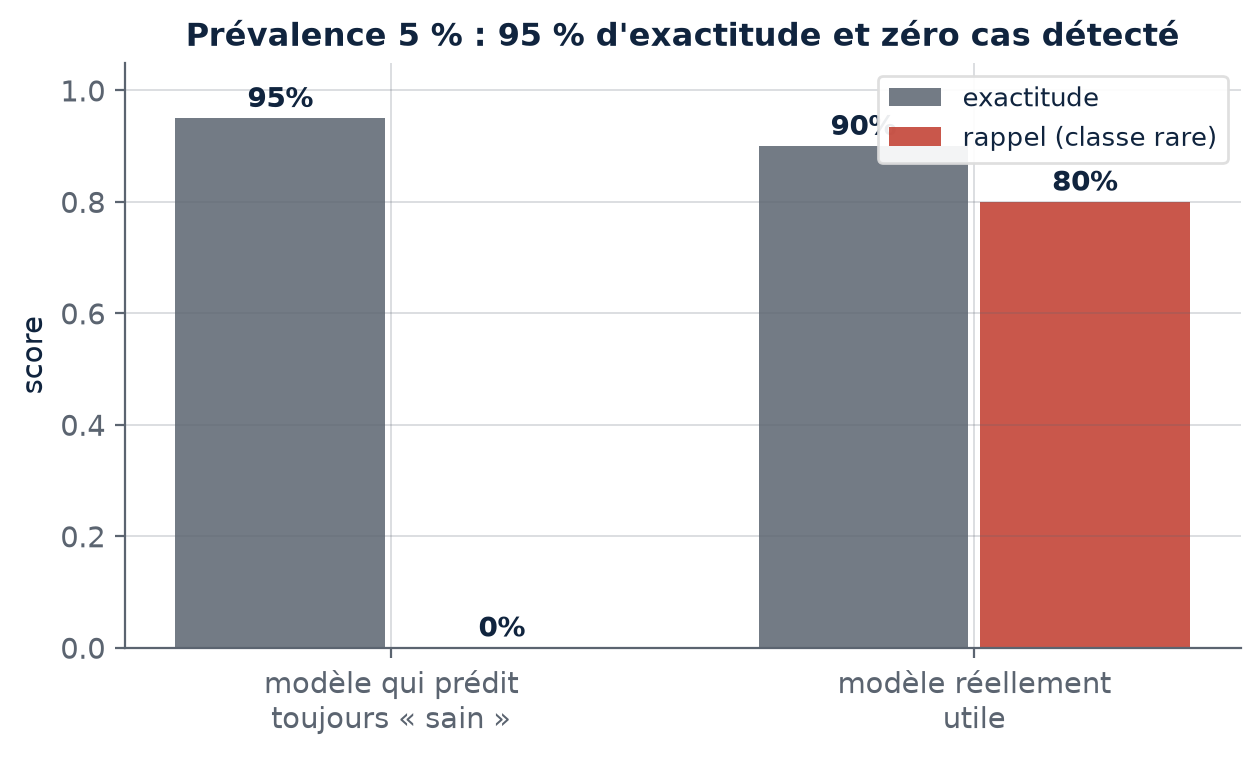
\includegraphics[height=0.32\textheight,keepaspectratio]{g11_desequilibre.png}
\end{column}
\begin{column}{0.52\textwidth}
\begin{itemize}
  \item Prévalence 5 \% : prédire toujours « sain » donne
        \textbf{95 \% d'exactitude} et \textbf{0 \% de rappel}.
  \item Un modèle utile : \textbf{90 \%} d'exactitude, \textbf{80 \%} de rappel.
  \item Le second est « moins bon » sur le papier, et infiniment plus utile.
\end{itemize}
\begin{wbox}[Conséquence]
Sur des classes rares, jamais l'exactitude seule : précision, rappel et $F_1$.
\end{wbox}
\end{column}
\end{columns}
\end{frame}

\begin{frame}{Les remèdes, par ordre de coût}
\begin{center}
\small
\begin{tabular}{@{}p{0.26\textwidth}p{0.28\textwidth}p{0.34\textwidth}@{}}
\toprule
\textbf{Symptôme} & \textbf{Remède} & \textbf{Coût} \\
\midrule
Surapprentissage & plus de données & collecte, souvent le plus cher \\
 & augmentation / régularisation & immédiat \\
 & modèle plus simple & gratuit \\
Sous-apprentissage & variables plus informatives & ingénierie \\
 & modèle plus expressif & temps de calcul \\
Écart irréductible & changer de problème & à assumer \\
\bottomrule
\end{tabular}
\end{center}
\vspace{1.5mm}
\begin{kbox}[Régularisation, en une ligne]
Ajouter à la perte un terme $\lambda\lVert\theta\rVert^2$ (Ridge) ou
$\lambda\lVert\theta\rVert_1$ (Lasso) pénalise la complexité : on échange un
peu de biais contre beaucoup de variance. $\lambda$ se règle sur la validation.
\end{kbox}
\end{frame}

\begin{frame}{Des types de données aux représentations}
\begin{center}
\small
\begin{tabular}{@{}p{0.16\textwidth}p{0.32\textwidth}p{0.40\textwidth}@{}}
\toprule
\textbf{Donnée} & \textbf{Forme de $X$} & \textbf{Ce que cela impose} \\
\midrule
Tabulaire & matrice $n \times d$ & peu de prétraitement, modèles à arbres
adaptés \\
Texte & séquences de longueur variable & tokenisation, vocabulaire,
représentation vectorielle \\
Image & tenseur $H \times W \times C$ & convolutions, augmentation \\
Série temporelle & $n$ observations ordonnées & découpage temporel, décalages \\
\bottomrule
\end{tabular}
\end{center}
\vspace{1.5mm}
\begin{kbox}[Le choix du modèle suit la structure]
Un tableau se traite bien par arbres ou modèles linéaires ; une image par
convolutions ; une série par décalages ou modèles séquentiels. Appliquer un
modèle inadapté coûte plus cher que mal régler un modèle adapté.
\end{kbox}
\end{frame}

\begin{frame}[fragile]{Du concept au code : le pipeline}
\begin{codebox}[Pipeline minimal, sans fuite]
\begin{lstlisting}
from sklearn.model_selection import train_test_split, cross_val_score
from sklearn.pipeline import Pipeline
from sklearn.preprocessing import StandardScaler
from sklearn.linear_model import LogisticRegression

Xtr, Xte, ytr, yte = train_test_split(X, y, test_size=0.2,
                                      stratify=y, random_state=42)

modele = Pipeline([("sc", StandardScaler()),
                   ("clf", LogisticRegression(max_iter=1000))])

scores = cross_val_score(modele, Xtr, ytr, cv=5)   # reglages
modele.fit(Xtr, ytr)
print(scores.mean(), modele.score(Xte, yte))       # test, une seule fois
\end{lstlisting}
\end{codebox}
\vspace{1mm}
{\footnotesize Le \texttt{Pipeline} garantit que la standardisation est
réajustée dans chaque pli : c'est la traduction opérationnelle de la règle
« rien ne doit voir le test ».
}
\end{frame}

\begin{frame}[fragile]{Ce que fait réellement « entraîner »}
\begin{columns}[t]
\begin{column}{0.48\textwidth}
\begin{codebox}[Boucle d'apprentissage]
\begin{lstlisting}
for epoque in range(n_epoques):
    y_pred = modele(X)
    perte  = perte_fn(y_pred, y)
    perte.backward()      # gradients
    optimiseur.step()     # theta <- theta - eta * grad
    optimiseur.zero_grad()
\end{lstlisting}
\end{codebox}
\end{column}
\begin{column}{0.48\textwidth}
\begin{kbox}[Les quatre gestes, toujours les mêmes]
\begin{enumerate}
  \item prédire ;
  \item mesurer la perte ;
  \item calculer le gradient ;
  \item descendre d'un pas.
\end{enumerate}
\end{kbox}
\begin{wbox}[Ce qui change d'un modèle à l'autre]
Le calcul du gradient et la forme de $\theta$ --- pas la boucle.
\end{wbox}
\end{column}
\end{columns}
\end{frame}

\begin{frame}{Validation croisée imbriquée (pour aller plus loin)}
\begin{columns}[t]
\begin{column}{0.50\textwidth}
\begin{itemize}
  \item \textbf{Boucle externe} : estime la performance.
  \item \textbf{Boucle interne} : choisit les hyperparamètres.
  \item Chaque pli externe refait sa propre sélection.
\end{itemize}
\begin{wbox}[Pourquoi ce détour]
Régler $\lambda$ sur les mêmes plis qui servent à évaluer rend le score
optimiste : c'est une fuite par sélection, exactement comme choisir les
variables avant le split.
\end{wbox}
\end{column}
\begin{column}{0.46\textwidth}
\begin{solbox}[Coût]
$K_{\text{ext}} \times K_{\text{int}} \times G$ entraînements, où $G$ est la
taille de la grille. Inutile pour un modèle unique, indispensable dès qu'on
compare plusieurs réglages.
\end{solbox}
\begin{kbox}[Ordre des opérations]
Sélectionner \emph{dans} le pli, évaluer \emph{sur} le pli. Jamais l'inverse.
\end{kbox}
\end{column}
\end{columns}
\end{frame}

\begin{frame}{Activité : choisir la métrique (8 min)}
\begin{abox}[Trois situations --- quelle métrique, et pourquoi ?]
\begin{enumerate}
  \item \textbf{Dépistage} d'une maladie rare : rater un malade coûte cher.
  \item \textbf{Filtre anti-spam} : un courriel légitime bloqué exaspère
        l'utilisateur.
  \item \textbf{Prévision de la demande} pour un stock : erreur en unités,
        quelques jours à l'avance.
\end{enumerate}
\end{abox}
\vspace{1mm}
\begin{solbox}[Réponses attendues]
\textbf{1.} Rappel élevé (quitte à accepter des fausses alertes).
\textbf{2.} Précision élevée (peu de faux positifs).
\textbf{3.} MAE ou RMSE, comparée à une persistance.
\end{solbox}
\end{frame}

\begin{frame}{Étude de cas : le projet à 99 \%}
\begin{wbox}[La situation]
Un groupe annonce \textbf{99 \% d'exactitude} pour repérer les étudiants en
difficulté. Le notebook révèle trois choix :
\begin{itemize}
  \item la colonne « a été convoqué en tutorat » a été conservée comme variable ;
  \item le découpage est aléatoire alors qu'un même étudiant apparaît sur
        plusieurs semestres (quasi-doublons) ;
  \item sept modèles ont été essayés, et le meilleur score sur le test est
        celui qui est annoncé.
\end{itemize}
\end{wbox}
\vspace{1mm}
\begin{abox}[À traiter en binôme (10 min)]
\begin{enumerate}
  \item Identifier la nature exacte de chaque fuite.
  \item Estimer l'ordre de grandeur du score honnête.
  \item Rédiger les trois exigences à imposer au groupe avant validation.
\end{enumerate}
\end{abox}
\end{frame}

\begin{frame}{Quiz 3 --- formalisation et évaluation}
\begin{columns}[t]
\begin{column}{0.49\textwidth}
\begin{qbox}[Question 1]
$\hat R_n(\theta)$ est :
\begin{itemize}
  \item[(a)] la performance sur la population
  \item[(b)] la performance sur l'échantillon
  \item[(c)] la perte de l'optimum
\end{itemize}
\end{qbox}
\begin{qbox}[Question 2]
Un pas d'apprentissage trop grand provoque :
\begin{itemize}
  \item[(a)] un surapprentissage
  \item[(b)] une divergence de l'optimisation
  \item[(c)] une fuite de données
\end{itemize}
\end{qbox}
\end{column}
\begin{column}{0.49\textwidth}
\begin{qbox}[Question 3]
Sur 5 \% de positifs, 95 \% d'exactitude et 0 \% de rappel signifie :
\begin{itemize}
  \item[(a)] un bon modèle
  \item[(b)] un modèle qui prédit toujours la classe majoritaire
  \item[(c)] une erreur de calcul
\end{itemize}
\end{qbox}
\begin{solbox}[Réponses]
\textbf{1.} (b). \quad \textbf{2.} (b). \quad \textbf{3.} (b).
\end{solbox}
\end{column}
\end{columns}
\end{frame}

\begin{frame}{À retenir et TP}
\begin{kbox}[Les cinq idées du chapitre]
\begin{enumerate}
  \item Apprendre $=$ minimiser le risque empirique dans une famille $\mathcal{H}$.
  \item L'écart entre risque empirique et risque réel est le vrai sujet du cours.
  \item Un modèle trop riche mémorise ; trop pauvre, il ne peut pas représenter.
  \item Le découpage doit reproduire l'usage réel : temporel, stratifié, sans fuite.
  \item Toute métrique se lit avec sa baseline et son incertitude.
\end{enumerate}
\end{kbox}
\vspace{1.5mm}
\begin{abox}[TP1 : \file{notebooks/TP1_premier_pipeline.ipynb}]
Pipeline complet : découpage, baseline, régression logistique, matrice de
confusion, validation croisée, puis fabrication d'une fuite et mesure de son
effet. Durée : \textbf{2 h} · barème : \textbf{10 points}.
\end{abox}
\end{frame}
